% $Id$ 
%==============================================================================
\section{A Nested Component's Structure}
%==============================================================================

\begin{figure}[htb]
    \begin{center}
    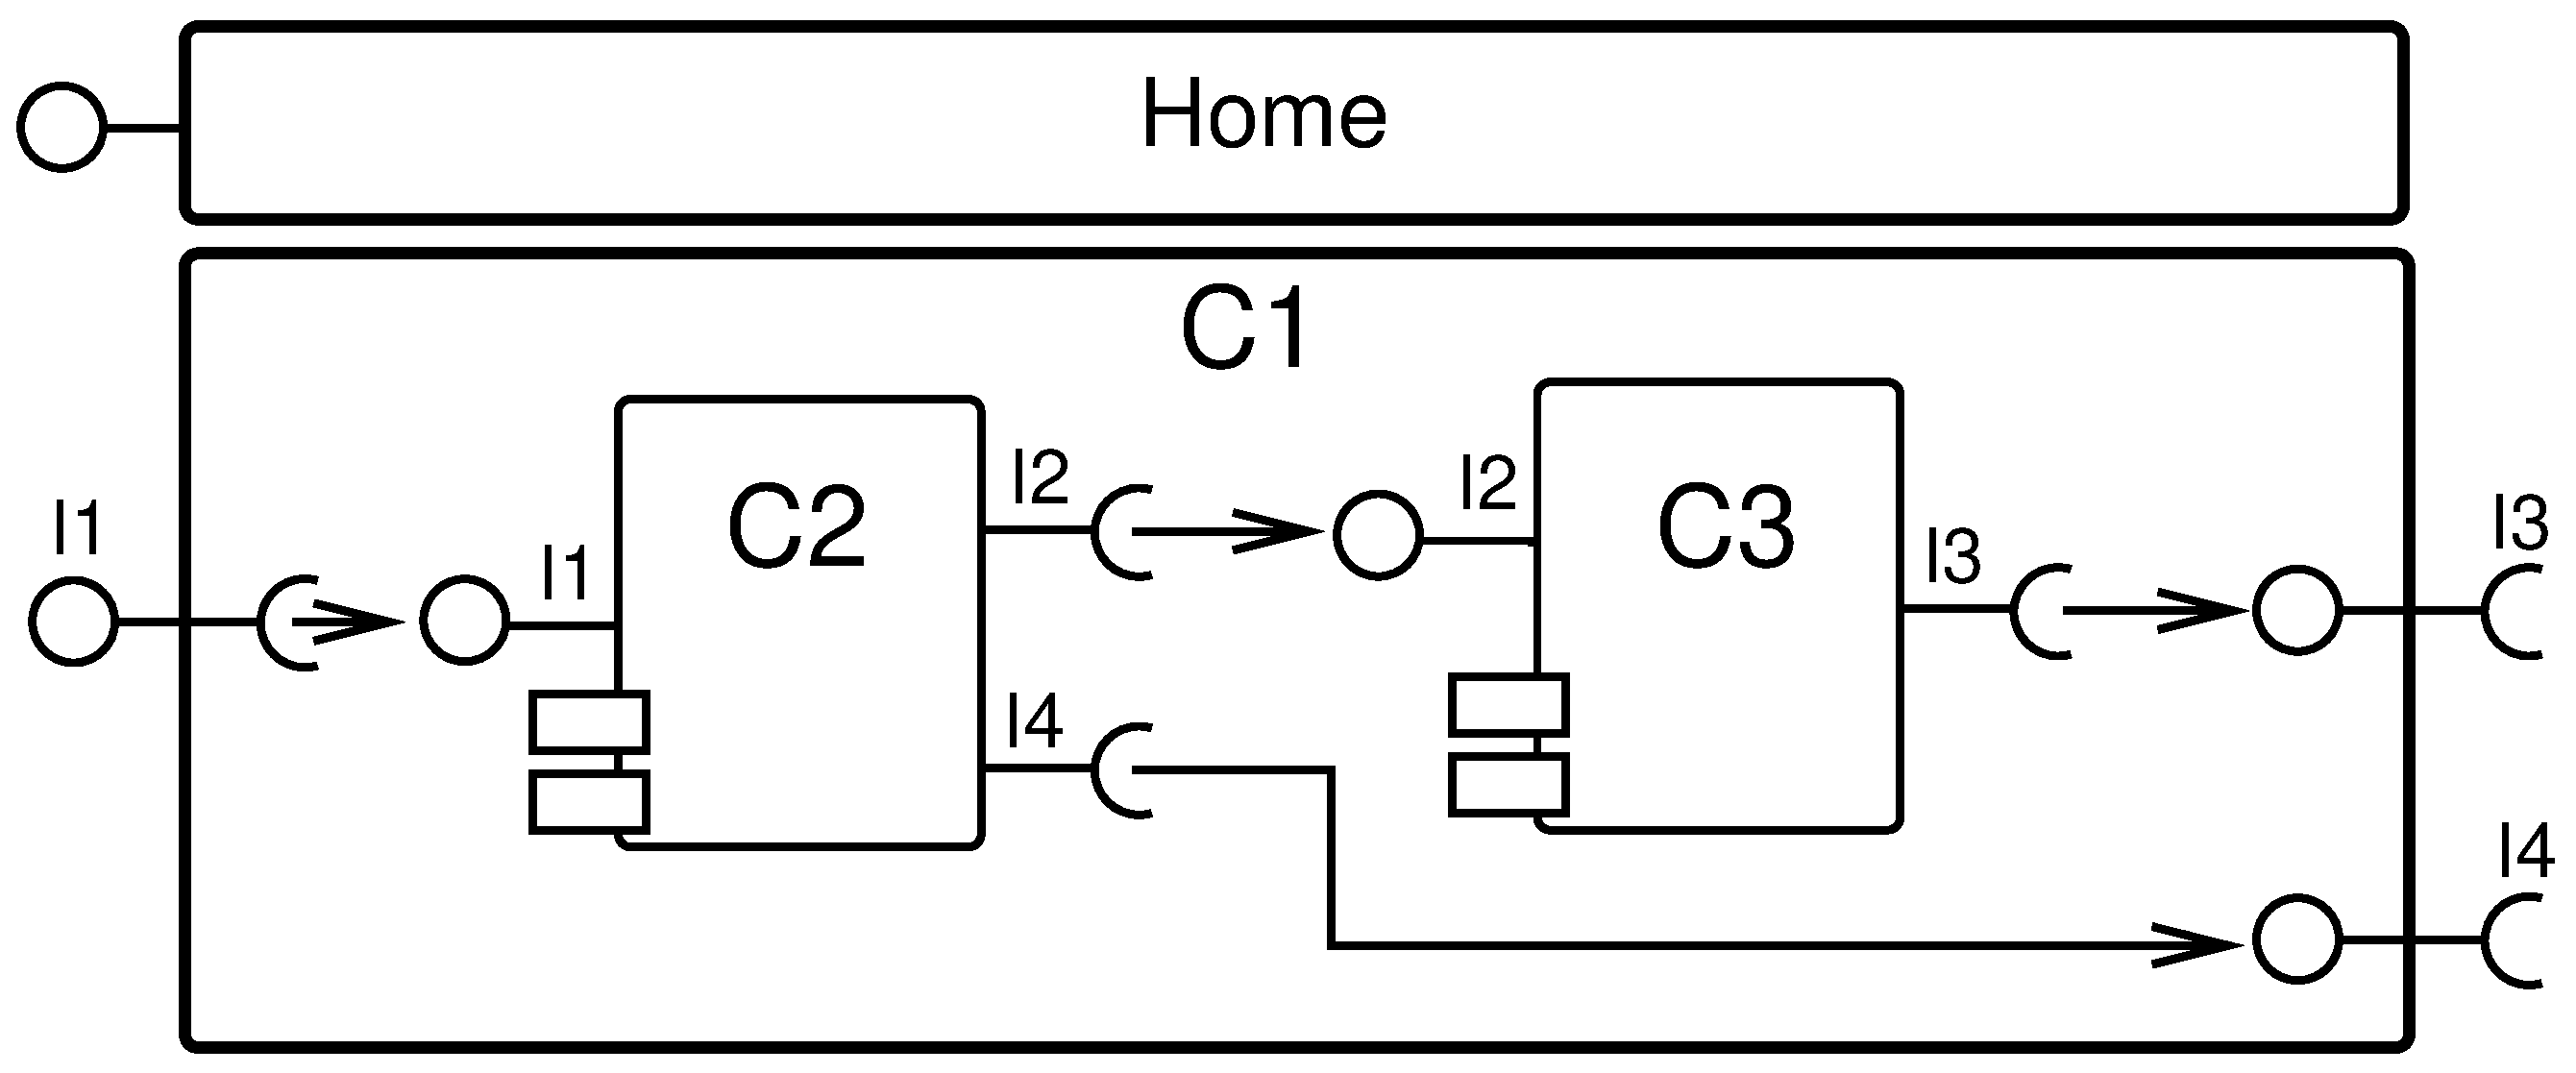
\includegraphics [width=7cm,angle=0] {figures/NestedAssembly.eps}
    \caption{ $C_{Ref}$ super component example.}
    \label{NestedAssembly}
    \end{center}
\end{figure}

Using the session facade pattern \cite{J2EECorePatterns}, 
we are able reduce a nested component composition into a flat component 
assembly that can be described by a simple CAD file.
While the inner components $C2$, $C3$ keep unchanged, the outer component $C1$ 
must be transformed into a special LwCCM component - the facade component, 
as shown in Fig.~\ref{NestedToFlatAssembly}.

\begin{figure}[htb]
    \begin{center}
    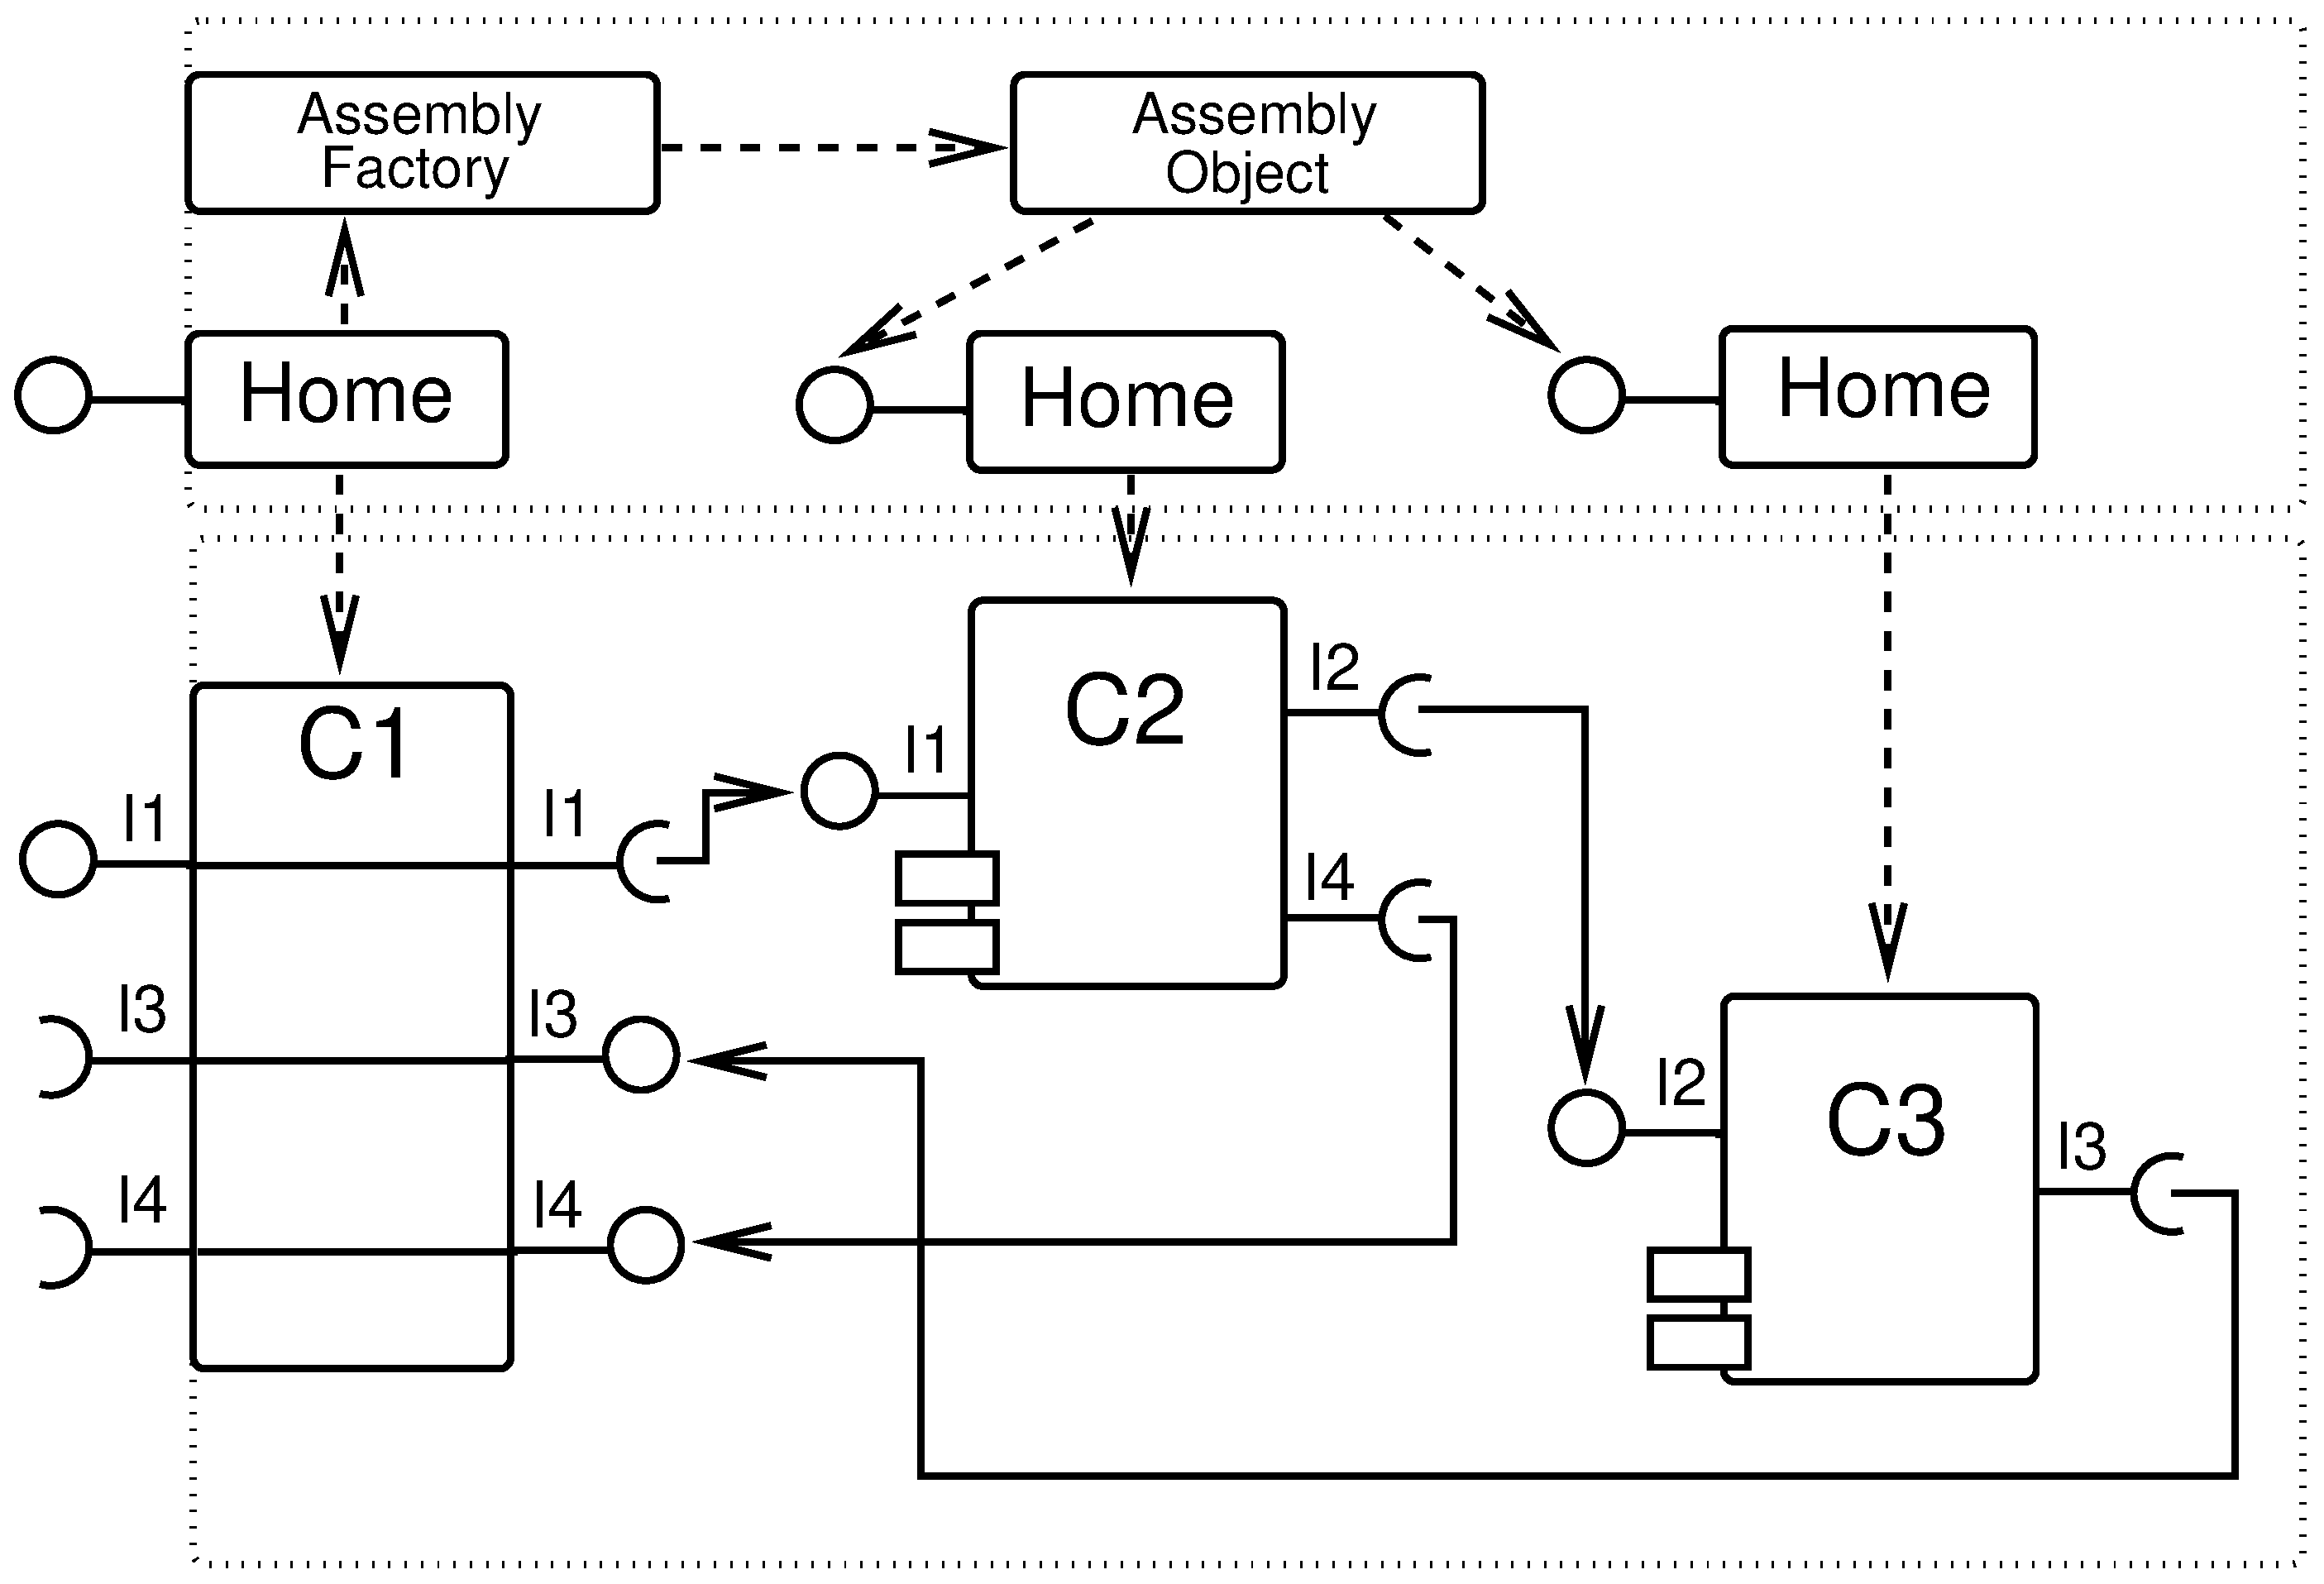
\includegraphics [width=7cm,angle=0] {figures/NestedToFlatAssembly.eps}
    \caption{Using the session facade pattern, a nested component composition
    can be reduced to a flat assembly as defined in LwCCM.}
    \label{NestedToFlatAssembly}
    \end{center}
\end{figure}

\noindent
The LwCCM facade component provides two complementary kinds of ports for each 
port defined in $C1$:
\begin{itemize}
\item {\bf Public ports.} A public port is visible to component clients and
can be accessed as a regular LwCCM component port.
 
\item {\bf Private ports.} A private port is a LwCCM port that is
not visible to component clients.
Private ports are used to connect the facade component with their inner 
component instances.
Technically, private ports are implemented like public ports, but after the
configuration phase, private ports can not be accessed by component clients. 
\end{itemize}
 
\noindent
All information about components and their connections within a super 
component are represented by an {\it Assembly Object}.
Such an assembly object is assigned to a facade component instance, and 
can be seen as a part of the facade component itself. 

For each facade component instance, an instance of the corresponding assembly
object must be created. 
To give a facade component's home the ability to create assembly object 
instances, an {\it Assembly Object Factory} must be assigned to a facade 
component home during component deployment.
With this approach, we can use regular LwCCM components and assemblies
to realize the nested component concept.

The implementation of a facade component's business logic is straightforward, 
each call to a facet method delegates to the corresponding receptacle and 
vice versa.

\vspace{3mm}
\noindent
To give a client the illusion of a single component, a facade component has to
handle some tasks behind the scenes. These are defined by the following 
sequence diagrams. 

\begin{figure}[htb]
    \begin{center}
    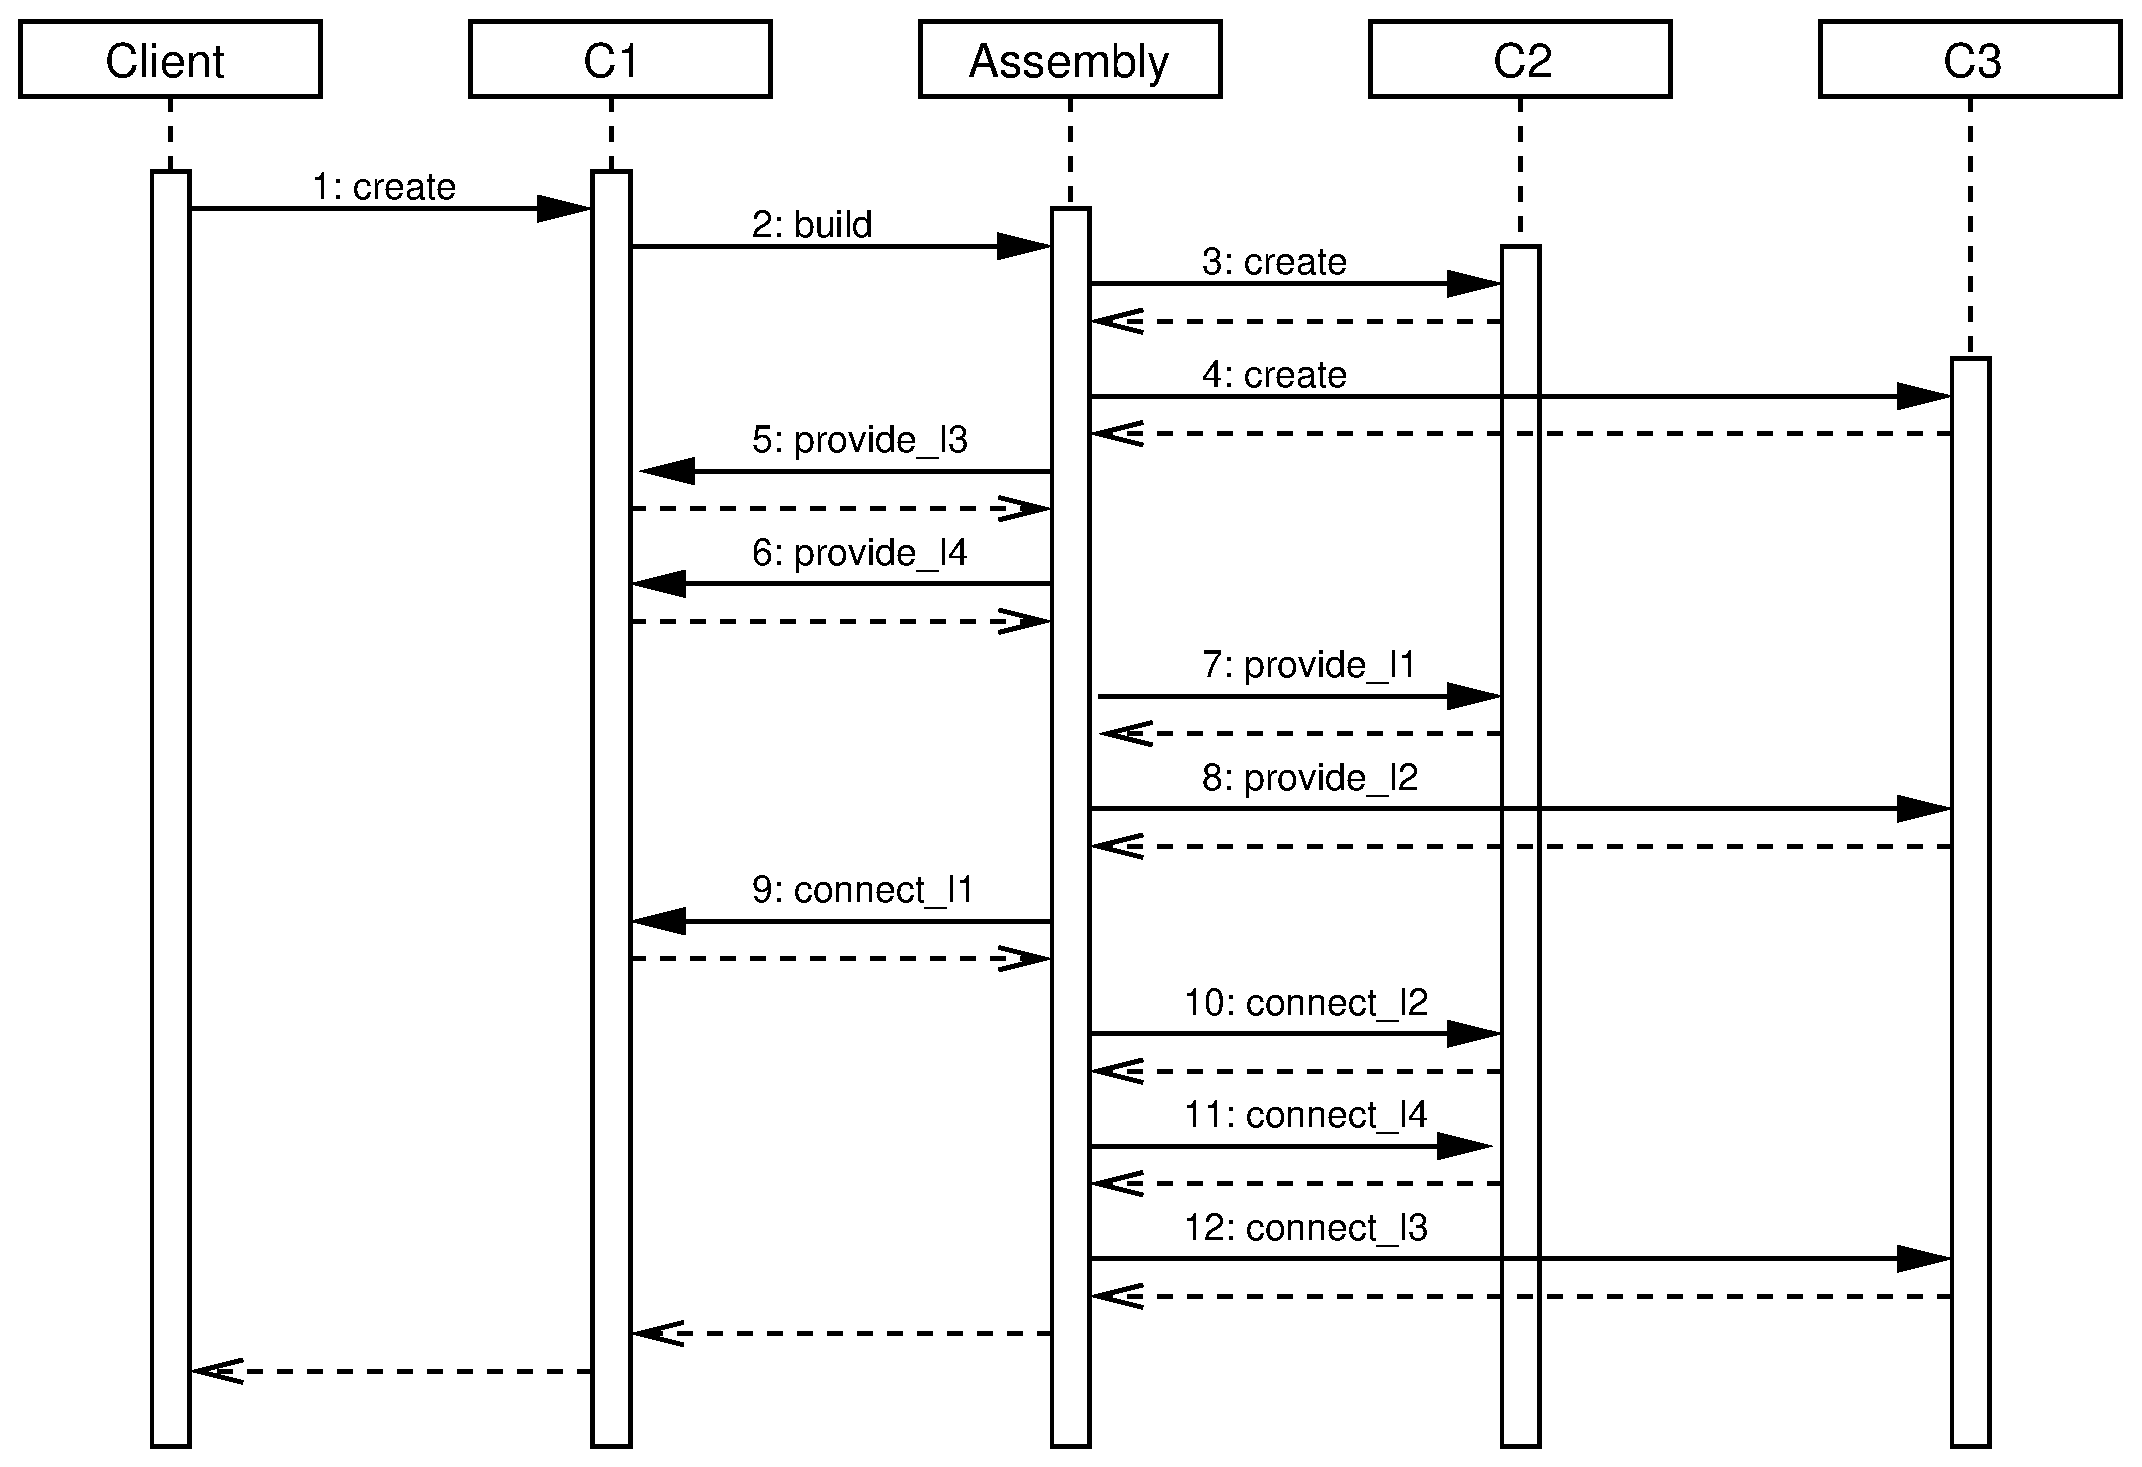
\includegraphics [width=12cm,angle=0] {figures/SuperComponentCreate.eps}
    \caption{Create a super component of Fig~\ref{NestedToFlatAssembly}.}
    \label{SuperComponentCreate}
    \end{center}
\end{figure}

\noindent
From a client's point of view, there is only one component $C_1$ that can be
instantiated by $C_1$'s home (Fig.~\ref{SuperComponentCreate}).
In fact, $C_1$ calls the {\tt build} method of the associated assembly object.
This assembly object in turn instantiates $C_2$ and $C_3$ and establishes all 
defined connections between these component instances.
After these activities, the assembly object returns to $C_1$ that finishes 
its create method.

Of course, $C_1$ itself can be part of another super component or connected 
to other components as well.
LwCCM defines the end of a component's configuration phase by calling the
{\tt configuration\_complete} method on each component instance.
In the case of a super component, this call must be delegated to all 
subcomponent instances (Fig.~\ref{SuperComponentConfigurationComplete}).
Before $C_1$ can return from {\tt configuration\_complete}, it has to lock all
private ports to prevent clients from directly accessing contained component 
instances.

\begin{figure}[htb]
    \begin{center}
    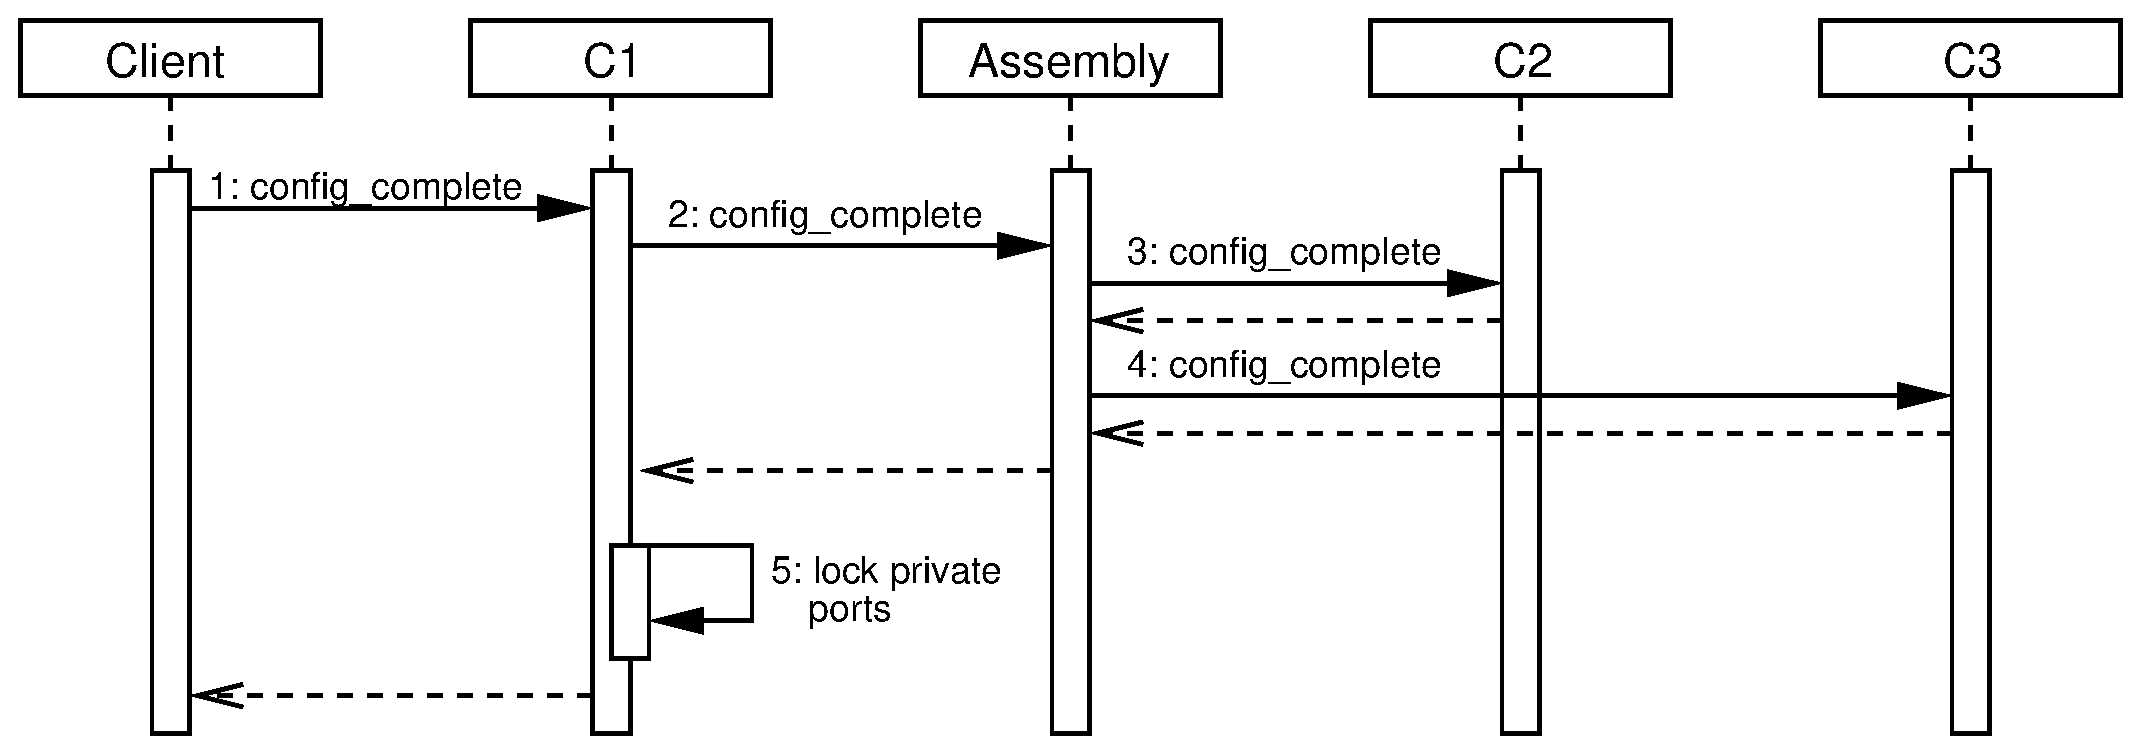
\includegraphics [width=12cm,angle=0] 
		     {figures/SuperComponentConfigurationComplete.eps}
    \caption{Completion of super component configuration phase.}
    \label{SuperComponentConfigurationComplete}
    \end{center}
\end{figure}

\noindent
Fig.~\ref{SuperComponentRemove} shows how a super component instance is removed:
$C_1$ triggers the assembly object to disconnect and destroy
all contained component instances.

\begin{figure}[htb]
    \begin{center}
    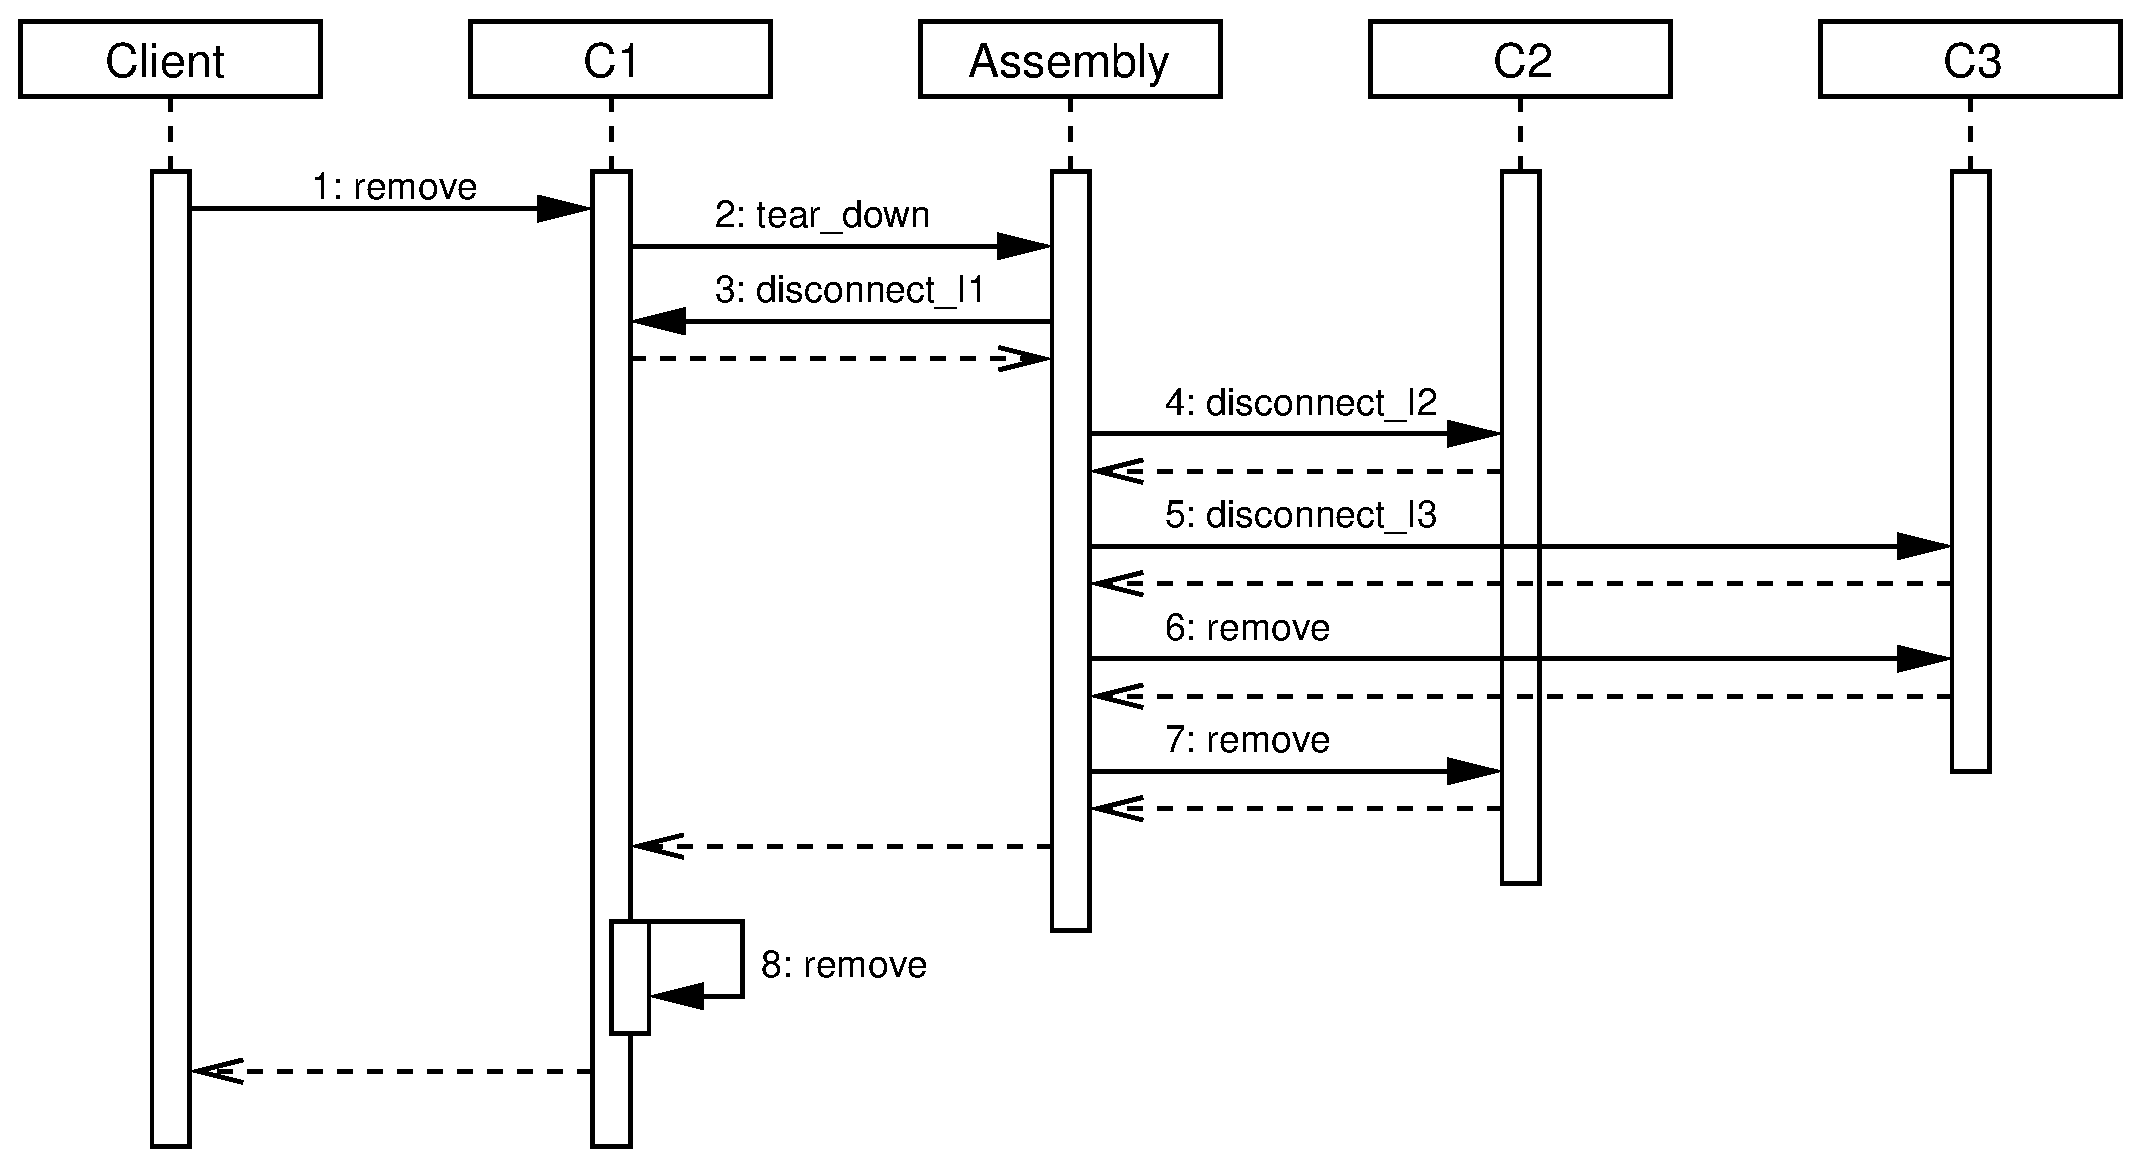
\includegraphics [width=12cm,angle=0] {figures/SuperComponentRemove.eps}
    \caption{Removal of a super component.}
    \label{SuperComponentRemove}
    \end{center}
\end{figure}

\noindent
A component client can handle
the super component in the same way as a regular LwCCM component.
Also, a simple LwCCM component can be seen as a special case of a super
component with an empty assembly.
Thus, both components and assemblies has been reduced to a single concept.

